\documentclass{beamer}
\usepackage{presentation}

\begin{document}

\frame{\titlepage}

\begin{frame}
  \frametitle{Need and goal statement}

  What we
  \textbf{need}:
  \input{build/need_statement_md}
  \newline
  \newline
  Our
  \textbf{goal}:
  \input{build/goal_statement_md}

\end{frame}

\begin{frame}
  \frametitle{Design Objectives}

  Four key objectives:
  \begin{itemize}
    \item Presence
    \item Portability / ease of set-up
    \item Configurable
    \item Accessible
  \end{itemize}

\end{frame}

\begin{frame}
  \frametitle{What our project could have been...}

  Map task management methods to devices, generate unique ideas
  \newline
  \newline

  \begin{columns}
    \column{0.5\textwidth}
    Method
    \begin{itemize}
      \item Personal assistant
      \item Accountability
      \item Streaks, levels
      \item Planner
    \end{itemize}

    \column{0.5\textwidth}
    Device
    \begin{itemize}
      \item Home assistant
      \item Face tracking sprayer
      \item Game device
      \item PDA Device
    \end{itemize}

  \end{columns}

\end{frame}

\begin{frame}
  \frametitle{Choosing the best design}

  We derived weights from our daily use of electronics and apps

  \begin{longtable}[]{@{}ll@{}}
  \toprule
  Criteria & Weight \\
  \midrule
  \endhead
  Budget & 20 \\
  Presence & 20 \\
  Ease of Use & 20 \\
  Barrier of Entry & 20 \\
  Sustainability & 10 \\
  Privacy & 10 \\
  \bottomrule
  \end{longtable}

  \note[item]{Explain what each of these mean}
  \note[item]{Connect weights with decision chart}
  \note[item]{Show how these weights apply to the products shown in the previous slide}

\end{frame}

\begin{frame}
  \frametitle{Embedded System Flow}

  \begin{center}
    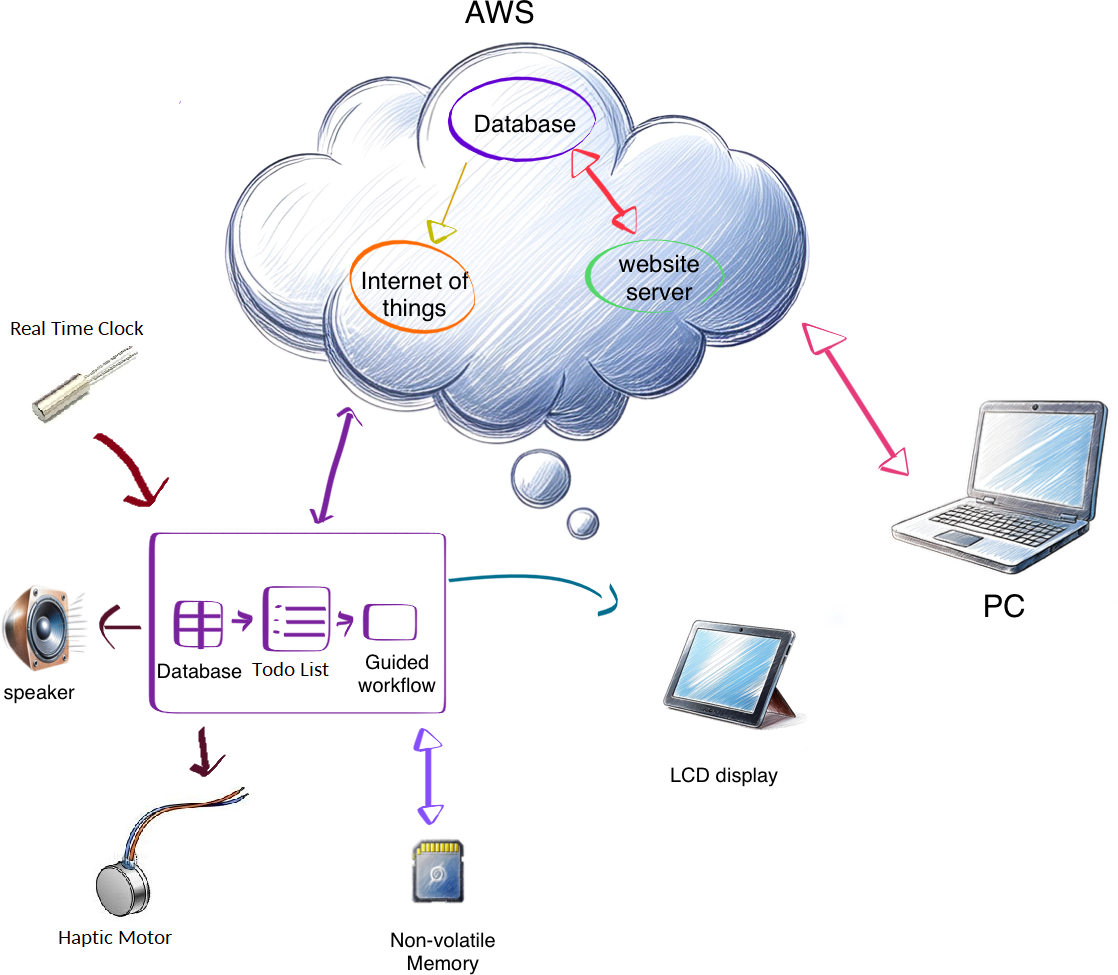
\includegraphics[height=0.7\textheight]{embedded_system_flow_chart.png}
  \end{center}

  \hfill {\tiny Source: Apple Playground for images}

  \note[item]{AWS IoT provides MQTT connection with esp32}
  \note[item]{Simple Storage Service (S3) provides database}
  \note[item]{Elastic Compute Cloud (EC2) provides web server}
  \note[item]{Web server with Flask + boto3 (S3 SDK) on python, nginx for the actual server, all on docker}
  \note[item]{Audio, LCD, and storage will be managed by their own components}
  \note[item]{Everything will be running as a FreeRTOS task with some shared resources}

\end{frame}


\begin{frame}
  \frametitle{Testing}

  \begin{columns}
    \column{0.7\textwidth}
    Testing on the microcontroller can be automated with Unity and pytest.
    \newline
    \newline
    For physical and software tests, we will define the following:
    \begin{itemize}
      \item Stimulus
      \item Control variables
      \item Expected Results
      \item Walkthrough of the procedure
    \end{itemize}

    \column{0.3\textwidth}
    
\includegraphics[width=0.5\textwidth]{pytest_logo.png} \\
    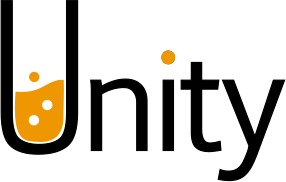
\includegraphics[width=0.5\textwidth]{unity_logo.png}

  \end{columns}

  \hfill {\tiny Source: pytest docs, Unity homepage}
  \note[item]{Unity for unit testing functions}
  \note[item]{pytest for automating tests on the target}
  \note[item]{Mention testing for areas outside areas defined by software - durability, user experience, etc.}
\end{frame}

\begin{frame}
  \frametitle{Prototype}

  \begin{center}
    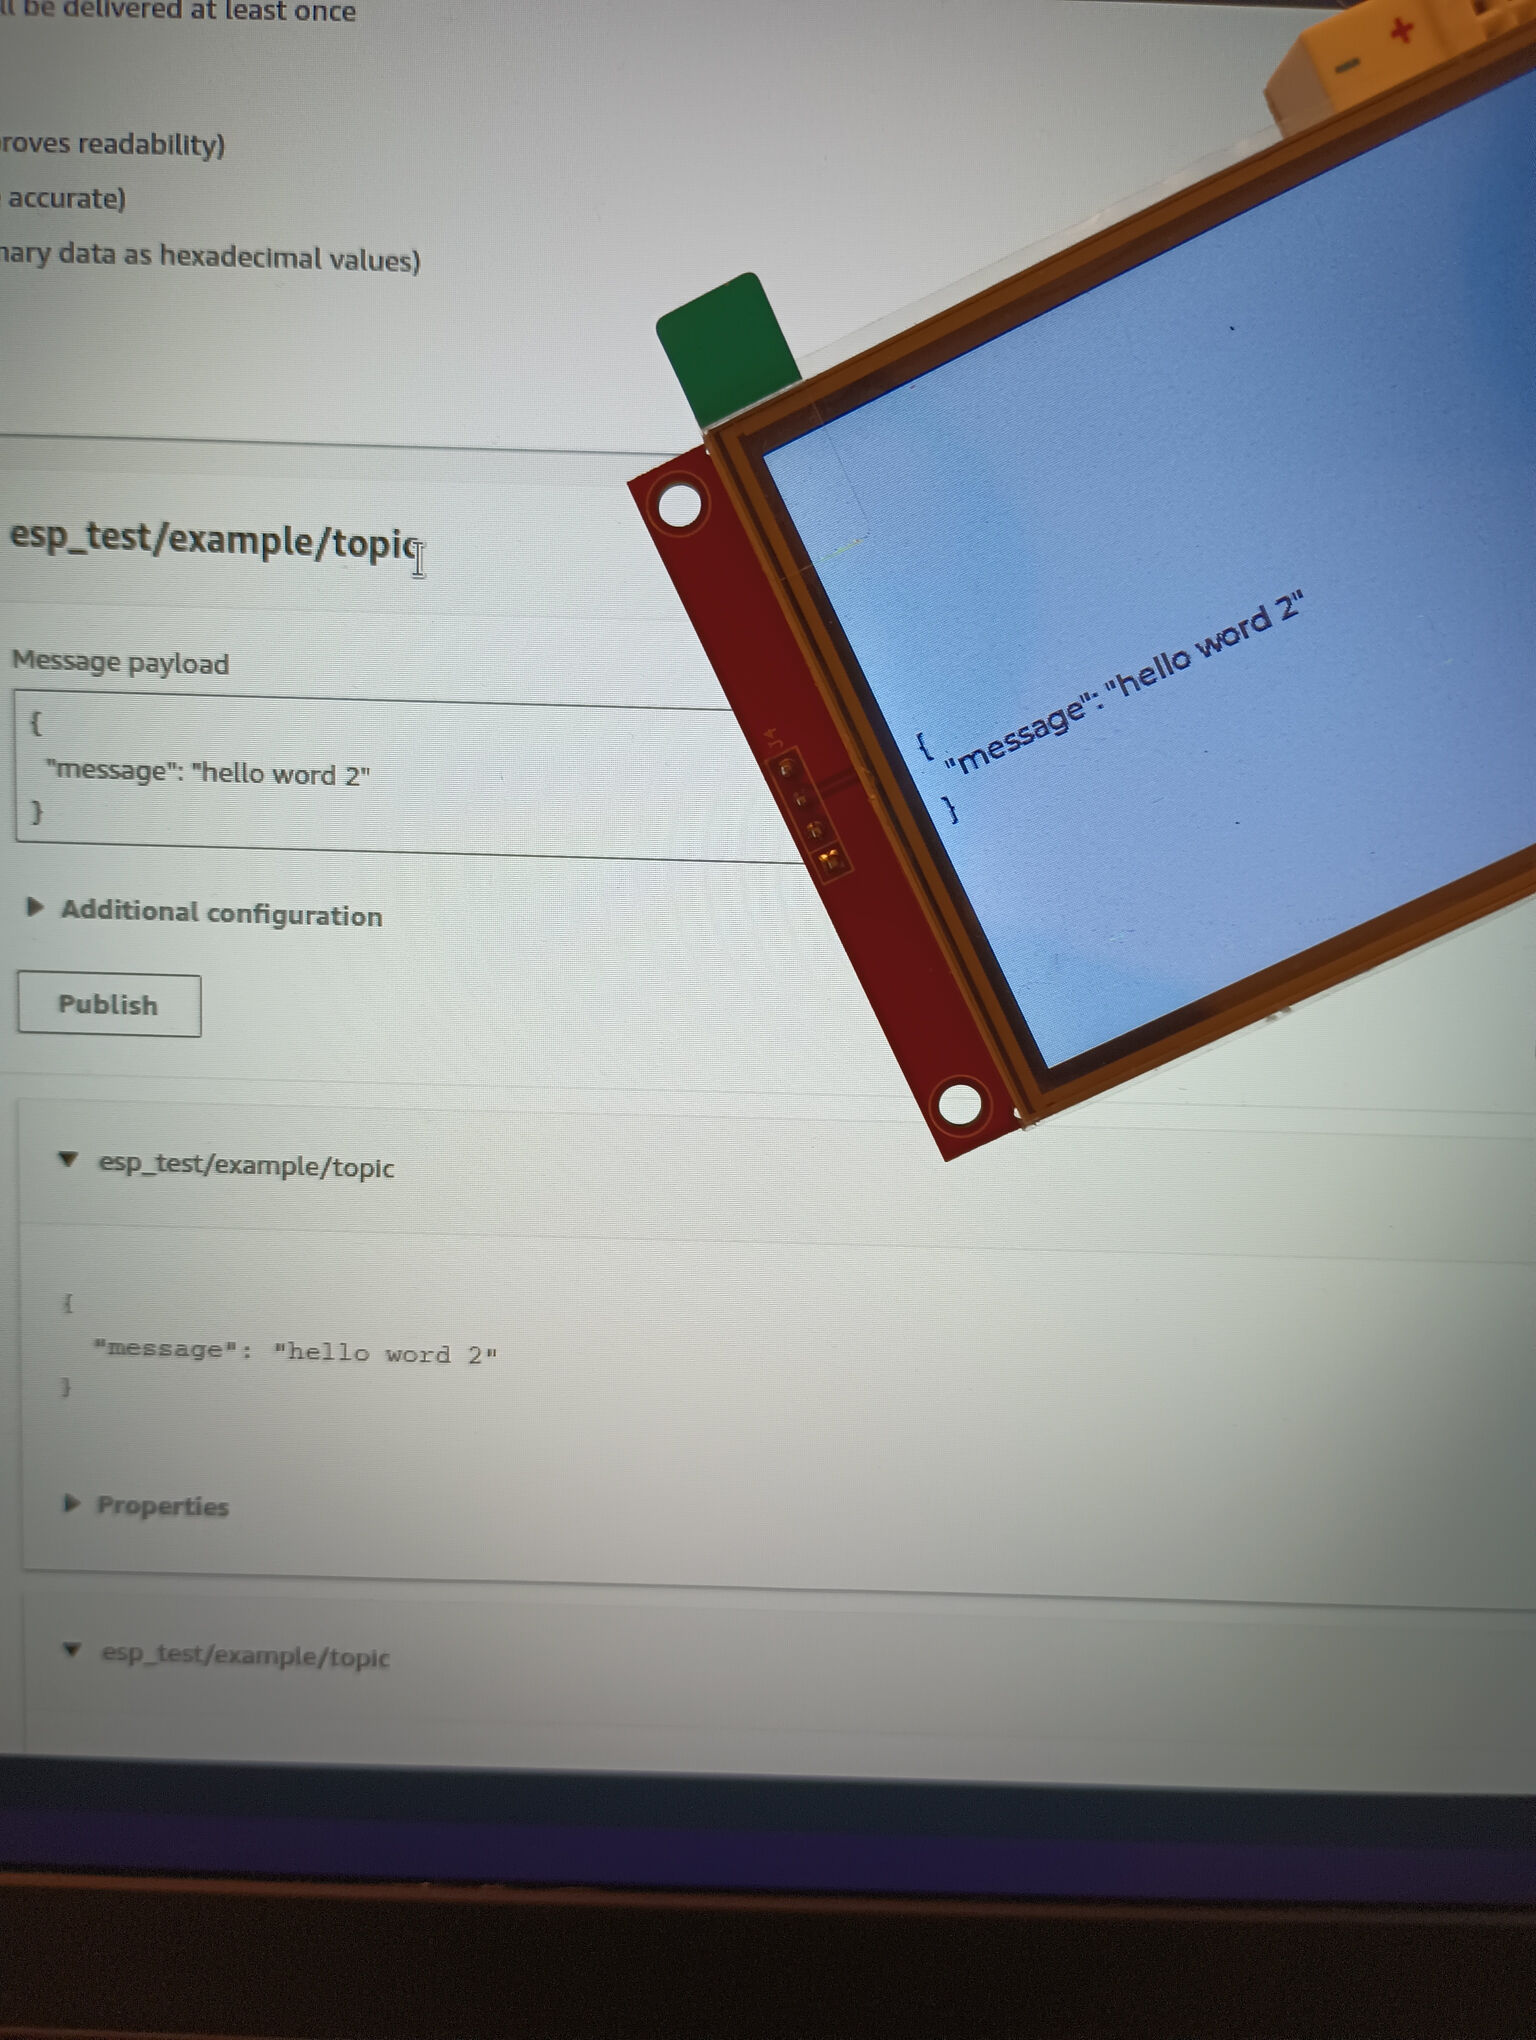
\includegraphics[height=0.7\textheight]{aws_demo.jpg}
  \end{center}

\end{frame}

\begin{frame}
  \frametitle{Algorithm Overview}
  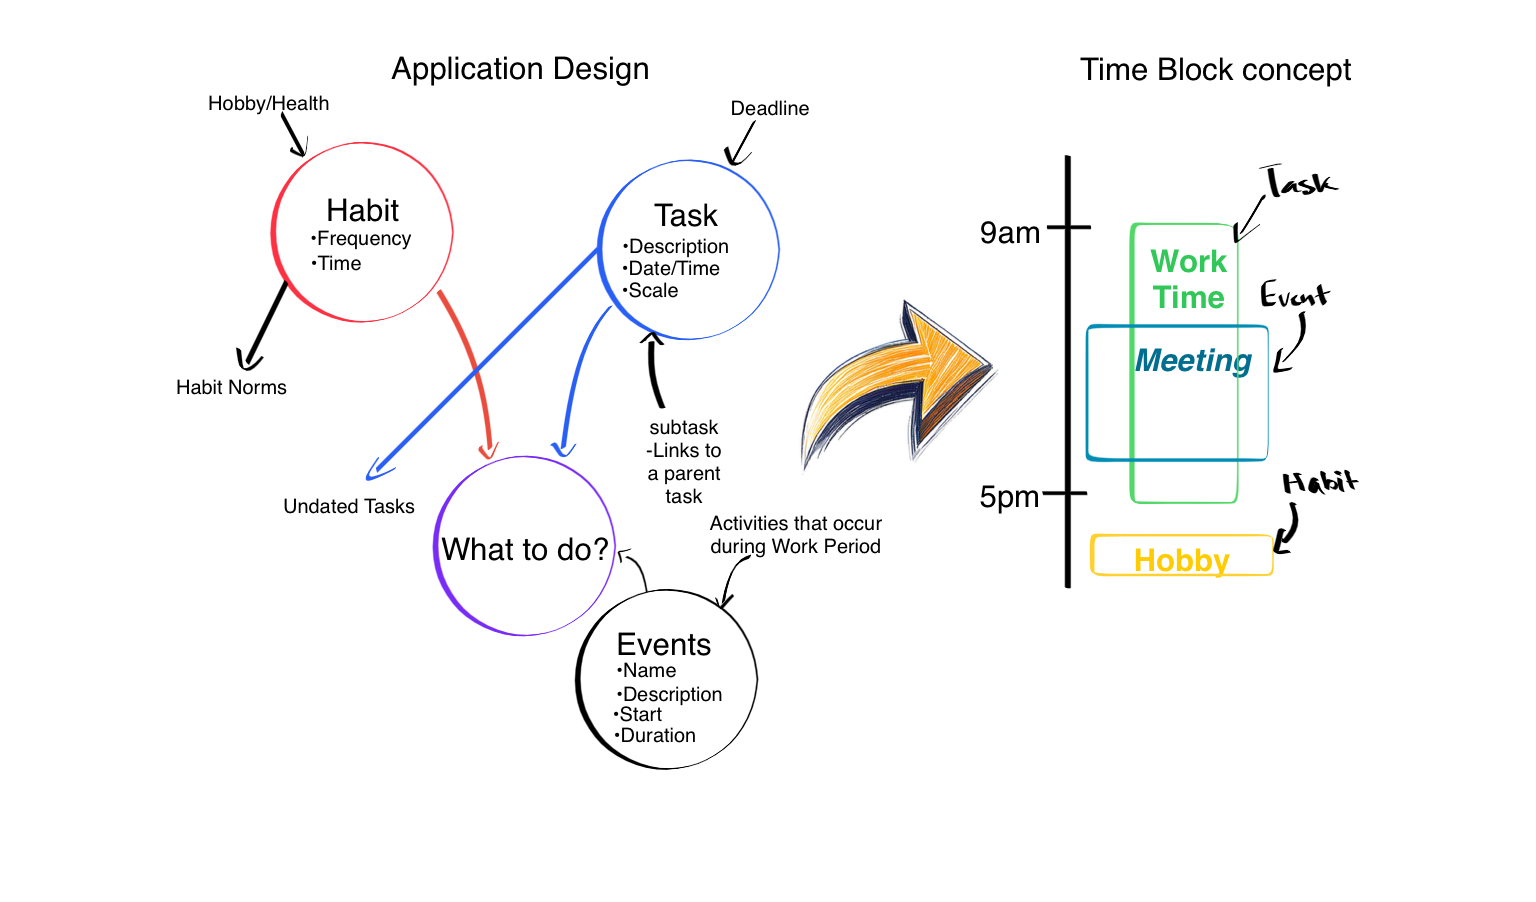
\includegraphics[width=\textwidth]{design_logic.png}
\end{frame}

\begin{frame}
  \frametitle{What's next?}
  % Confidence on on-time completion
  \begin{itemize}
    \item Unit testing with each module
    \item Database management software
  \end{itemize}
\end{frame}

\end{document}
